% INTRODUÇÃO-------------------------------------------------------------------

\chapter{INTRODUÇÃO}
\label{chap:introducao}

% Importância de estudar o CNV
A variação no número de cópias (Copy Number Variation/CNVs) é um dos fatores que contribuem para a expansão e diversidade da família de genes, ela foi observada como alterações ocorridas em larga escada de inserções, deleções e duplicações na região genômica \cite{Perry2009,Zhao2013,Redon2006,Costain2016}. 
As CNVs podem ser identificada como uma variação neutra ou como modificadores de sucessibilidade a doenças \cite{Costain2016,Perry2009}.

% Estratégia de identificar CNV e ligação a doenças
A análise da região genômica pode ser realizada graças as tecnologias desenvolvidas para seu o sequenciamento, permitindo a observação de variantes de DNA \cite{Sathirapongsasuti2011}. Embora o sequenciamento completo do genoma seja uma abordagem utilizada para a investigação de CNVs, uma estratégia mais viável, econômica e eficiente no tempo para o estudo da base genética da doença é o sequenciamento completo do exoma, sendo que 85\% dos variantes ligados a doenças mendelianas são encontrados nele \cite{Chong2015,Sathirapongsasuti2011,Fromer2012}.

% Ligação aos modelos estatísticos
Devido a quantidade, complexidade e ruído dos dados obtidos a partir sequenciamento das regiões codificantes do genoma (exoma), muitos ferramentas de detecção de CNVs foram desenvolvidos para determinar os tipos, quantidades e a localização de variações \cite{Fromer2012,Tan2014}. Esses fatores foram alcançados devido a utilização de modelos estatísticos na descoberta de variações no mapa de dados gerados no sequenciamento do exoma, essa é uma das abordagens que obteve mais sucesso na integração das ferramentas com o sequenciamento devido a sua eficiência \cite{Tan2014}.

A utilização de modelos estatísticos aplicados para detecção de \textit{copy number variation} visa encontrar pontos de mudanças em uma representação gráfica dos dados, assim facilitando a determinação de uma variação de acordo com a localização do ponto de mudança \cite{Zhao2013}. Essa técnica se tornou popular, sendo desenvolvidos diversas ferramentas que detecta pontos de mudanças (Change Point Detection/CPD) focadas na análise de CNV \cite{Olshen2004,Baldi2001,Girimurugan2018,Picard2011,Plagnol2012,Muggeo2010}. 

Apesar das diversas técnicas e ferramentas existentes de CPD, nenhuma delas é capaz de identificar todas as CNVs presentes no exoma \cite{Zhao2013}, entretanto a utilização de algumas dessas técnicas em determinada situação alcança uma maior efetividade ao encontrar as variações. Essa diferença entre as técnicas pode ser vista ao comparar a execução de cinco algoritmos específicos de detecção de variações no números de cópias na \autoref{fig:ferramentas-cnv} \cite{Muggeo2010}.

\begin{figure}[!htb]
    \centering
    \caption{Segmentação da linha celular de câncer de mama MDA157, onde cada linha representa um cromossomo, indexado ao lado esquerdo}
    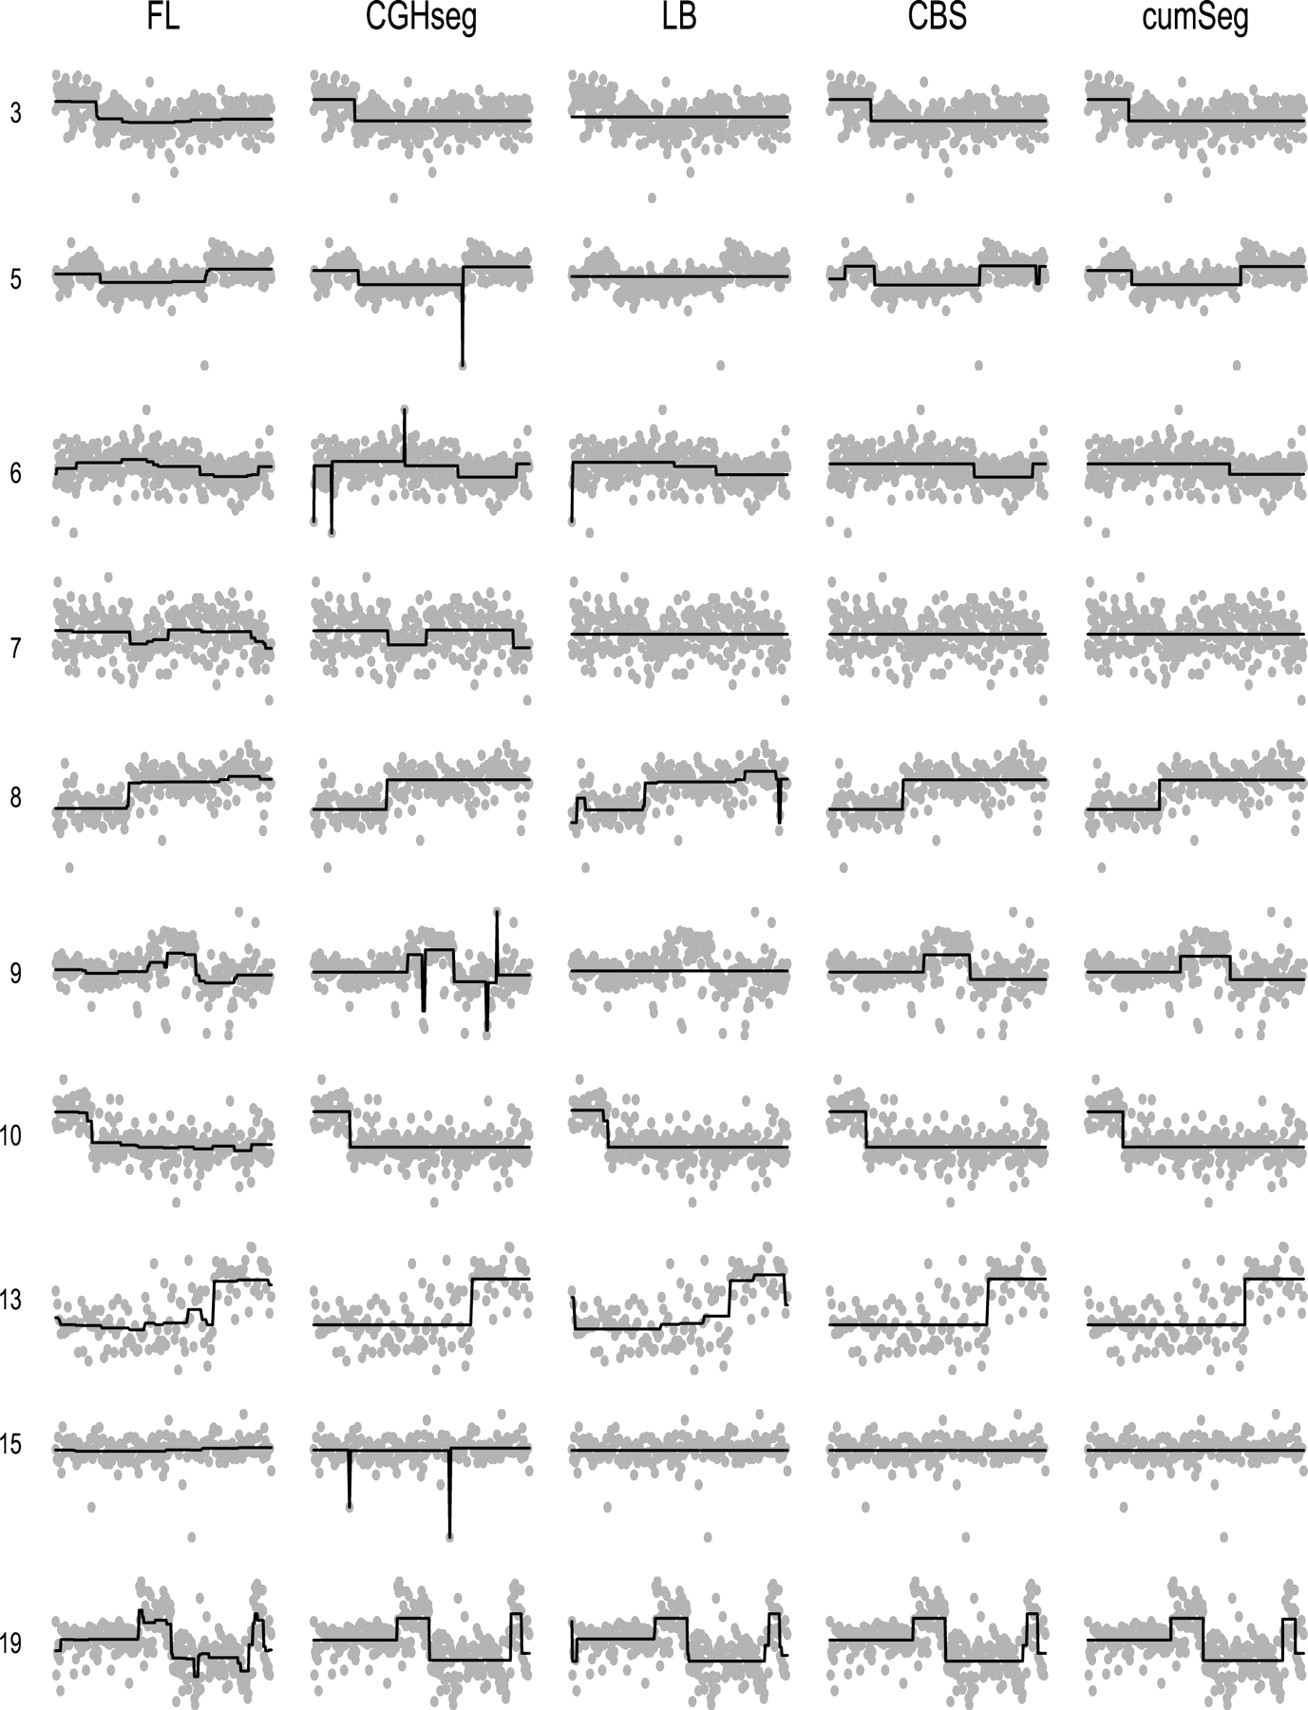
\includegraphics[width=0.8\textwidth]{./dados/figuras/ferramentas-cnv}
    \fonte{\cite{Muggeo2010}}
    \label{fig:ferramentas-cnv}
\end{figure}


% Contextualizar do estudo de CNV

% O genoma é uma grande fonte de informações acerca das nossas características e hereditariedade \cite{Correa2008}. O estudo das pequenas frações de regiões codificadoras de proteína do genoma (exoma) é bastante importante para a análise de doenças de origem genética, pois nele é contido cerca de 85\% de variantes conhecidos ligados a doenças \cite{Chong2015}.

% O exoma pode ser extraído por meio de um sequenciamento, onde seus variantes ficam visíveis para aplicação de algoritmos de análises e estudo de especialistas (referencia). O avanço tecnológico para detecção de padrões e anomalias nos dados gerados a parti do exoma tem-se evoluído ao longo do tempo, permitindo a observação das variações dos números de cópias (CNV) de cromossomos no DNA (referencia).

% A partir do sequenciamento do exoma é possível realizar uma distribuição dos dados mapeados em um gráfico, assim originando uma série temporal, ou seja, um conjunto de dados distribuídos ao longo de um determinado tempo (referencia). Desta forma, aumentando viabilidade de se analisar o CNV em determinadas posições.

% O Copy Number Variation (CNV) é observado quando ocorre alguma inserção ou deleção no cromossomo, fazendo com que ele deixe de ser diploide (referencia). Com a distribuição do dataset gerado pelo sequenciamento do exoma em um gráfico, os CNV ficam visíveis para serem estudados, mas a identificação do ponto onde ocorre algum tipo de CNV não é fácil de ser apontado e ou classificado, assim dificultando o apontamento de doenças genéticas.

% O reconhecimento da mudança ou ponto de mudança com uma maior precisão é um dos grandes desafios relacionado a análise estatística (referencia). O CP é fundamental para dar continuidade em pesquisas relacionadas a doenças ocorridas por algum CNV (referencia).

% O \textit{Change Point} é pouco perceptível a olho nu, dificultando o seu reconhecimento com uma maior precisão. Embora haja algoritmos que o detectam, como por exemplo \textit{Circular Binary Segmentation} ele não possui uma performance adequada para analise das segmentações mais recentes, pois elas contém uma quantidade imensa de marcadores assim aumentando o número de cálculos necessários para identificar a mudança em um determinado ponto por causa do uso de permutação em seu algoritmo.

% No meio estatístico, existe a utilização e implementação de diversos cálculos para solucionar tal questão, como  

% Diante das questões expostas, a exploração de novas algoritmos capaz de demonstrar uma melhor apresentação para detectar o CP vem sendo estudada, tanto no meio da estatística quanto no da bioinformática (referencia). Mas com a evolução e melhora das tecnologias, temos cada vez mais nitidez nas extração dos dados do exoma, assim necessitando de algoritmos e técnicas mais potentes para inspeção.

\section{JUSTIFICATIVA}



\section{OBJETIVOS}

Nesta seção será apresentado os objetivos que esse trabalho busca ao ser desenvolvido, sendo composto pelo objetivo geral e específico.

\subsection{Objetivo Geral}

Aplicar o conceito de detecção de pontos de mudanças, utilizando diferentes abordagens técnicas desenvolvidas para segmentação de dados de uma série temporal para anotação de variações no números de cópias nos dados do sequenciamento do exoma.

\subsection{Objetivos Específicos}
	
\begin{itemize}
    \item Explicar a importância de \textit{copy number variation}.
    \item Descrever o conceito de \textit{change point detection}, caracterizando com exemplos, os algoritmos desenvolvidos para esse objetivo.
    \item Analisar a aplicabilidade dos algoritmos de CPD para a CNV, citando exemplos dos mesmos.
\end{itemize}

\section{ORGANIZAÇÃO DO TEXTO}

Este trabalho se organiza da seguinte forma:

\autoref{chap:introducao} - Introdução: Situa o leitor na área de pesquisa em que o trabalho é focado, definindo o porque do seu desenvolvimento e os objetivos a serem alcançados com a conclusão do projeto.

\autoref{chap:fundamentacaoTeorica} - Revisão de Literatura: Apresenta uma pesquisa que contém conceitos e reflexões acerca dos principais conceitos referente ao trabalho proposto. Nele é apresentado temas relacionado ao trabalho proposto como a definição de exoma e a importância da utilização dele para descobertas de doenças (\autoref{sec:exoma}), o estudo acerca do surgimento e a evolução de tecnologias capazes de obter os componentes do genoma (\autoref{sec:sequenciamentoDoDna}), a definição de CNVs, ressaltando a importância do estudo e o uso dos métodos e ferramentas de detecção nessa variação genética (\autoref{sec:copyNumberVariation}), a formulação de uma das estratégias de detecção de CNV, a detecção de pontos de mudanças, sendo apresentado algoritmos específicos para utilização nesse tipo de situação (\autoref{sec:changePointDetection}) e a conceituação de matriz de confusão para aplicação em estudos com o objetivo de analise de performance \autoref{sec:matrizDeConfusao}.

\autoref{chap:planoDeTrabalho} - Plano de Trabalho: Expõe o cronograma adotado para o desenvolvimento do trabalho, disponibilizando o inicio e fim de um conjunto de atividades e sua descrição.

\autoref{chap:conclusao} - Conclusão: Apresenta as considerações finais acerca do trabalho desenvolvido.